\documentclass{article}
\usepackage{graphicx} 

\title{Problem Set 7}
\author{Steven Plaisance}
\date{March 2023}

\begin{document}

\maketitle

\begin{enumerate}
  \item Here we see the data summary output describing each numeric variable within the wages dataset. 25\% of logwage observations are missing. I think the missing observations are likely to be missing at random. 
  
  \linebreak
  \linebreak
      \parbox{\linewidth}{
        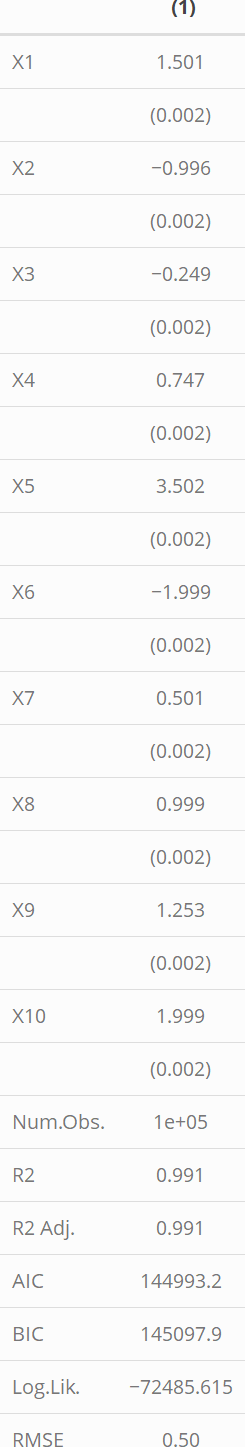
\includegraphics[width=14cm]{summaryTable.png}
        \centering
        \\}
  \item Here we see the model summary output of each of the four models. Beta 1 seems to decrease as we account for missing logwage observations, indicating that the data is likely not missing completely at random. It seems that the list-wise deletion model and the predicted value model performed most closely to the true value of Beta 1. The last two methods use a modeling approach to generate predictions for the missing observations based on the other variables. 
  
    \linebreak
    \linebreak
      \parbox{\linewidth}{
        \includegraphics[width=14cm]{modelTable.png}
        \centering
        \\}
        
  \item My project is still in the early stages, but I am happy with my premise and excited to continue working. I am using GPS data that we collect at my job with the football team. Specifically, my project is focused on calculating longitudinal and lateral acceleration values using athlete orientation and angle of motion. In terms of modeling approaches, machine learning is a likely choice due to the vast amount of data available to me. 
\end{enumerate}
\end{document}
